\documentclass{article}
\usepackage{graphicx}
\usepackage{amsmath}
\usepackage{enumitem}
\usepackage{float}
\usepackage{listings}
\usepackage{xcolor}
\usepackage[a4paper, margin=1in]{geometry}
\title{Homework 1}
\author{Steve Gillet}
\date{\today}

% Custom information
\newcommand{\className}{Course: Automatic Control Systems – ASEN 5114-001 – Spring 2025}
\newcommand{\professorName}{Professor: Dale Lawrence}
\newcommand{\taName}{Teaching Assistant: Anantha Dhruva}

\lstdefinestyle{matlabstyle}{
    language=Matlab,              % Specify the language
    basicstyle=\ttfamily\footnotesize\color{black}, % Code font
    keywordstyle=\color{blue}\bfseries, % Keywords in blue
    stringstyle=\color{green},    % Strings in green
    commentstyle=\color{magenta}, % Comments in magenta
    numbers=left,                 % Line numbers on the left
    numberstyle=\tiny\color{black},% Line number style
    stepnumber=1,                 % Line number increment
    breaklines=true,              % Line breaking
    frame=single,                 % Border around code
    backgroundcolor=\color{white},
    tabsize=4,                    % Tab size
    showstringspaces=false,       % Don't show spaces in strings
}

\begin{document}

\maketitle
\textit{
    "Due: Monday, February 3, 2025 at 11:59 pm on Canvas. Please assemble a single PDF file for
    submission that includes your Matlab/Simulink code/diagrams, plots, and explanations of your
    work and the results. Label sections to correspond with those in the assignment. Don’t make it
    difficult to locate the text/code/plots for each section."
}

\section*{1.}

\textit{
    "[10pts] Find the parameters $R_M$, $L_M$, $K_\tau$, $J_M$, and $K_B$ from the motor specification sheet, noting
    units. Also, find the total gear ratio N from the motor shaft to the load shaft, and estimate the
    load shaft moment of inertia $J_L$. Use these to quantify the parameters in the transfer function
    relating $V_P$ to $\Theta_L$. Also, estimate the potentiometer scale factor $K_S$ from the data file posted on Canvas."
}

\begin{figure}[H]
    \centering
    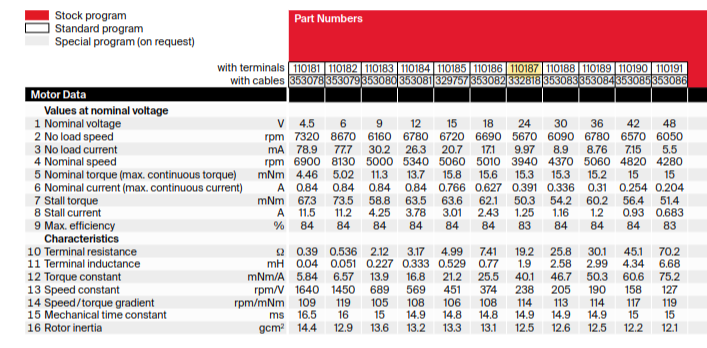
\includegraphics[width=0.9\textwidth]{motorSpec.png}
\end{figure}

I took the parameters from the motor specification table above using part number 110187.
\begin{align*}
    R_M&=19.2\;\Omega \\
    L_M&=1.9\text{mH}=0.0019\text{ H} \\
    K_\tau&=40.1\text{mNm/A}=0.0401\text{ Nm/A}  \\
    J_M&=12.5\text{gcm}^2=0.00000125\text{ kgm}^2 \\
    K_B&=238\text{rpm/V}=0.04\text{ Vs/rad} \\
    N&=3.3 \\
    J_L&=0.018522\text{ kgm}^2 \\
    K_S&=0.8
\end{align*}

I estimated $J_L$, using standard inertia formulas for a rod rotating about one end and a satellite (for the weight) and added them together.
\\
Equation for rod:
$J_{\text{arm}} = \frac{1}{3} m_{\text{arm}} L^2$
\\
Equation for weight:
$J_{\text{weight}} = m_{\text{weight}} L^2$
\\
\\
I got the mass of the arm and weight using their measurements and the average density for aluminum and brass.
\begin{itemize}
    \item Arm Dimensions: \( L = 30 \) cm, \( h = 0.7 \) cm, \( w = 1.1 \) cm
    \item Volume:
    \begin{equation}
        V_{\text{arm}} = L \times h \times w = 30 \times 0.7 \times 1.1 = 23.1 \text{ cm}^3
    \end{equation}
    \item Density of aluminum: \( \rho_{\text{Al}} \approx 2.7 \) g/cm³
    \item Mass of the arm:
    \begin{equation}
        m_{\text{arm}} = V_{\text{arm}} \times \rho_{\text{Al}} = 23.1 \times 2.7 = 62.37 \text{ g} = 0.0624 \text{ kg}
    \end{equation}
\end{itemize}

\begin{itemize}
    \item Weight Dimensions: \( 3.2 \times 2.0 \times 3.4 \) cm
    \item Volume:
    \begin{equation}
        V_{\text{brass}} = 3.2 \times 2.0 \times 3.4 = 21.76 \text{ cm}^3
    \end{equation}
    \item Density of brass: \( \rho_{\text{brass}} \approx 8.5 \) g/cm³
    \item Mass of the brass weight:
    \begin{equation}
        m_{\text{brass}} = V_{\text{brass}} \times \rho_{\text{brass}} = 21.76 \times 8.5 = 184.96 \text{ g} = 0.185 \text{ kg}
    \end{equation}
\end{itemize}

Then I used those numbers (including length of arm for L) to calculate the moments of inertia and combine them.

\begin{equation}
    J_{\text{arm}} = \frac{1}{3} m_{\text{arm}} L^2
\end{equation}

\begin{equation}
    J_{\text{arm}} = \frac{1}{3} (0.0624) (0.30)^2 = 0.001872 \text{ kg}\text{m}^2
\end{equation}

\begin{equation}
    J_{\text{weight}} = m_{\text{weight}} L^2
\end{equation}

\begin{equation}
    J_{\text{weight}} = (0.185) (0.30)^2 = 0.01665 \text{ kg}\text{m}^2
\end{equation}

\begin{equation}
    J_L = J_{\text{arm}} + J_{\text{brass}}
\end{equation}

\begin{equation}
    J_L = 0.00187 + 0.01645 = 0.018522 \text{ kg}\text{m}^2
\end{equation}

    
\end{document}